%begin---------------------Settings---------------------------%
\documentclass[12pt,a4paper,UTF8]{article}
\usepackage{geometry}
	\geometry{left=2cm,right=2cm,top=3.2cm,bottom=2.8cm}
\usepackage{amsmath,paralist,enumitem,booktabs,multirow,graphicx,subfig,setspace,listings,lastpage}
\usepackage[colorlinks,
            linkcolor=blue,       
            anchorcolor=blue,  
            citecolor=blue,       
            ]{hyperref}
	\setlength{\parindent}{2em}
	\lstset{language=Python}
\usepackage{fancyhdr}
	\pagestyle{fancy}
	\lhead{C9}
	\rhead{SUPPLEMENTARY INFORMATION}
	\cfoot{Page \thepage/\pageref{LastPage}}
	\rfoot{\today}
	\renewcommand{\headrulewidth}{0.4pt}
	\renewcommand{\theenumi}{(\arabic{enumi})}

\renewcommand{\thefigure}{S\arabic{figure}}
\renewcommand{\thetable}{S\arabic{table}}


%%begin-----------------Reference-----------------------%%
\usepackage[hyperref=true,backend=biber,bibstyle=science,citestyle=numeric-comp,sorting=none,backref=true]{biblatex}
\addbibresource{REF.bib}
%%end-------------------Reference-----------------------%%

%end---------------------Settings---------------------------%



%%%%%%%%%%%%%%%%%%%%%%%%%%%%%%%%%%%%%%%%%%%%%%%%%%%%%%%%%%
%%%%%%%%%%%%%%%%%%%%%%%%%Document%%%%%%%%%%%%%%%%%%%%%%%%%%
%%%%%%%%%%%%%%%%%%%%%%%%%%%%%%%%%%%%%%%%%%%%%%%%%%%%%%%%%%


\begin{document}
%begin---------------------Infor and Catalog---------------------------%

\begin{center}
\LARGE\textbf{C9 Unravel the general characteristics of chaotic systems by exploring chaotic circuits}

\vspace{0.5em}
\large{SUPPLEMENTARY INFORMATION}
\end{center}

\noindent
\textbf{Experimenter:} Zweig, Wong 20980066 \\
\textbf{Participant:} Runbing Mo 20980131 \\
\textbf{Date:} 2022.05.11


\tableofcontents
\newpage
%end---------------------Infor and Catalog---------------------------%

%begin---------------------Materials and instruments---------------------------%
\section{Materials and instruments}
\begin{table}[htbp]
    \centering
    \caption{\textbf{Materials and instruments}}
        \begin{tabular}{llll}
            \toprule
            &Name &Total &Model and parameters \\
            \midrule
            &$Anaconda$	&1	&$version\ 4.10.3$    \\    
            &$Multisim$	&1	&$version\ 16.0$    \\    
            &$LTspice$	&1	&$version\ 17.0.34$    \\    
            &Breadboard	&1	&    \\   
            &Various Electric components	&	&(Details in next section)    \\   
            \bottomrule
        \end{tabular}
\end{table}	
%end---------------------Materials and instruments---------------------------%

%begin---------------------Exp.1---------------------------%

\section{Exp.1 Chua's circuit}
    \subsection{Main parameters}
        \subsubsection{Numerical calculation}
        Parameters of different patterns adopted in the numerical calculation are summarized in Tab. \ref{tab.1.1}.
        These parameters can also be explored in the Jupyter Notebook provided in the thesis.
            \begin{table*}[htbp]
                \centering
                \caption{\textbf{Parameters of different patterns, numerical calculation}}
                \label{tab.1.1}
                    \begin{tabular}{ccccc}
                        \toprule
                        pattern	&$m_1$	&$m_2$	&$\alpha$	&$\beta$ \\
                        \midrule
                        line	&-2.0	&-1.3	&26	&12	\\
                        limit ring	&-0.5	&1.0	&13	&13	\\
                        double attractors	&-1.1	&-0.7	&21	&36	\\
                        1st single attractor	&-1.1	&-0.7	&21	&31	\\
                        2nd single attractor	&-1.1	&-0.7	&21	&15	\\
                        \bottomrule
                    \end{tabular}
            \end{table*}

        \subsubsection{Simulation}
        To generate different chaotic patterns, we adjusted the resistance value of $R_7$.
        The different resistance values of the corresponding patterns for the two circuits are summarized in Tab. \ref{tab.1.2} and Tab. \ref{tab.1.3}, respectively.
            \begin{table*}[htbp]
                \centering
                \caption{\textbf{Parameters of different patterns, simulation of circuit I}}
                \label{tab.1.2}
                    \begin{tabular}{cc}
                        \toprule
                        $pattern$	&$R_7$ \\
                        \midrule
                        line	&$ 0.00\% \times 2k\Omega$	\\
                        limit ring	&$ 76.8\% \times 2k\Omega$	\\
                        double attractors	&$ 86.8\% \times 2k\Omega$	\\
                        1st single attractor	&$ 94.8\% \times 2k\Omega$	\\
                        2nd single attractor	&$ 96.0\% \times 2k\Omega$	\\
                        \bottomrule
                    \end{tabular}
            \end{table*}
            
            \begin{table*}[htbp]
                \centering
                \caption{\textbf{Parameters of different patterns, simulation of circuit II}}
                \label{tab.1.3}
                    \begin{tabular}{cc}
                        \toprule
                        $pattern$	&$R_7$ \\
                        \midrule
                        line	&$ 0.00\% \times 2k\Omega$	\\
                        limit ring	&$ 52.0\% \times 2k\Omega$	\\
                        double attractors	&$ 78.0\% \times 2k\Omega$	\\
                        1st single attractor	&$ 80.6\% \times 2k\Omega$	\\
                        2nd single attractor	&Missing	\\
                        \bottomrule
                    \end{tabular}
            \end{table*}

        \subsubsection{Experiment}
        We built the two circuits and adjusted the resistance value of $R_7$ to get different chaotic patterns.
        Parameters of electric components are summarized in Tab. \ref{tab.1.4}
        Different resistance value of corresponding patterns for the two circuits are summarized in Tab. \ref{tab.1.5} and Tab. \ref{tab.1.6}, respectively.
        
        \begin{table}[htbp]
            \centering
            \caption{\textbf{Parameters of electric components}}
            \label{tab.1.4}
                \begin{tabular}{llll}
                    \toprule
                    &Name &Total &Value \\
                    &$L_1$	&1	&$21.005 mH$    \\    
                    &$C_1$	&1	&$10.277 nF$    \\    
                    &$C_2$	&1	&$91.104 nF$    \\    
                    &$R_1$	&1	&$218.43 \Omega$    \\    
                    &$R_2$	&1	&$220.13 \Omega$    \\    
                    &$R_3$	&1	&$22.060k \Omega$    \\    
                    &$R_4$	&1	&$21.923k \Omega$    \\    
                    &$R_5$	&1	&$2.2012k \Omega$    \\    
                    &$R_6$	&1	&$3.2625k \Omega$    \\    
                    &$R_7$	&1	&$Max 1.9650k \Omega$    \\    
                    \bottomrule
                \end{tabular}
        \end{table}	

            \begin{table*}[htbp]
                \centering
                \caption{\textbf{Parameters of different patterns, experiment of circuit I}}
                \label{tab.1.5}
                    \begin{tabular}{cc}
                        \toprule
                        $pattern$	&$R_7$ \\
                        \midrule
                        line	&$0.00 \Omega$	\\
                        limit ring	&$1498.20 \Omega$	\\
                        double attractors	&$1880.32 \Omega$	\\
                        1st single attractor	&$1907.20 \Omega$	\\
                        2nd single attractor	&Misssing	\\
                        \bottomrule
                    \end{tabular}
            \end{table*}

            \begin{table*}[htbp]
                \centering
                \caption{\textbf{Parameters of different patterns, experiment of circuit II}}
                \label{tab.1.6}
                    \begin{tabular}{cc}
                        \toprule
                        $pattern$	&$R_7$ \\
                        \midrule
                        line	&$0.00 \Omega$	\\
                        limit ring	&$1408.01 \Omega$	\\
                        double attractors	&$1563.20 \Omega$	\\
                        1st single attractor	&$1661.41 \Omega$	\\
                        2nd single attractor	&$1802.03 \Omega$	\\
                        \bottomrule
                    \end{tabular}
            \end{table*}

%end---------------------Exp.1---------------------------%

%begin---------------------Exp.2---------------------------%

\section{Exp.2 Lorentz's circuit}
    \subsection{Main parameters}
    \subsubsection{Numerical calculation}
    Parameters for generating the Lorentz butterfly in the numerical calculation are summarized in Tab. \ref{tab.2.1}.
    These parameters can also be explored in the Jupyter Notebook provided in the thesis.
        \begin{table*}[htbp]
            \centering
            \caption{\textbf{Parameters of Lorentz butterfly, numerical calculation}}
            \label{tab.2.1}
                \begin{tabular}{cccc}
                    \toprule
                    $pattern$	&$\alpha$	&$\beta$    &$\gamma$ \\
                    \midrule
                    butterfly	&10.0	&28.0	&2.8	\\
                    \bottomrule
                \end{tabular}
        \end{table*}

    \subsubsection{Simulation}
    The simulation circuit (Fig. \ref{fig.2.1}) and the corresponding parameters (Fig. \ref{fig.2.2}) to generate the Lorentz butterfly in LTspice are shown below.
    This schematic referenced Jim's work, who kindly provided his schematic on his website(\href{http://www.chaotic-circuits.com/10-creating-lorenz-butterfly/}{www.chaotic-circuits.com}).    
    We especially thanks to him.
    \begin{figure}[htbp]
        \centering
        \subfloat[The schematic]{\label{fig.2.1}
        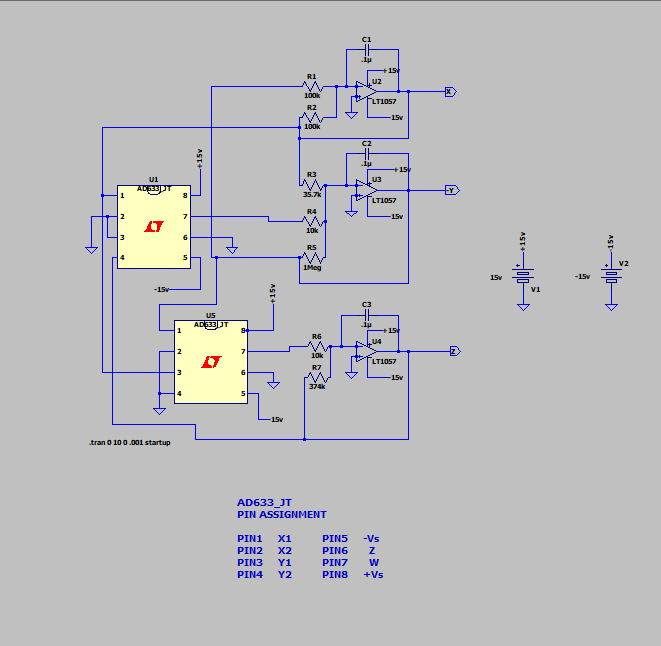
\includegraphics[width=0.3\textwidth]{attachments/fig.s2.1.png}
        }
        \subfloat[Parameters]{\label{fig.2.2}
        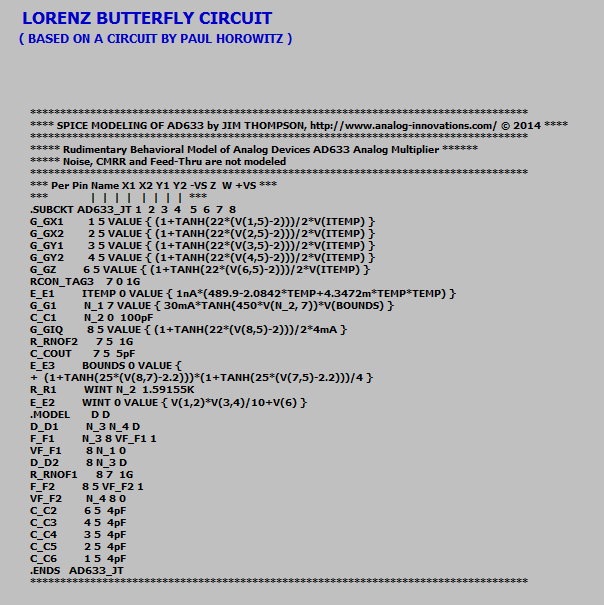
\includegraphics[width=0.3\textwidth]{attachments/fig.s2.2.png}
        }
        \caption{\textbf{Simulation of the Lorentz circuit}}
    \end{figure}

%end---------------------Exp.2---------------------------%


\section{Reflection question}
    \subsection{Application of chaotic circuits}
    \begin{enumerate}[label=\arabic*.]
        \item As mentioned in the thesis, when investigating other much more complex chaotic systems, it is a pretty effective way to create and operate on an electronic "analog" instead of directly working with the actual system, which may be difficult or impossible to control.
        \item Chaotic systems can be used for socalled chaos encryption, which means hiding data signals within a chaotic signal to ensure the security\autocite{tanougastHardwareImplementationChaos2011}. 
        \item They can also be used for true random bit generation taking advantages of their long-term unpredictability\autocite{nguimdoFastRandomBits2012a}. 
        \item In robotics, chaotic signals are being used in neural control networks or as chaotic path generators \autocite{steingrubeSelforganizedAdaptationSimple2010}.
    \end{enumerate}

\section{Data and code availability}
Data and code are available at \url{https://github.com/Zweig-Wong/SYSU-PHY-EXP}
%%begin--------------------Reference------------------------%%
\printbibliography[title=Reference] 
%%end--------------------Reference------------------------%%

\end{document}